\section{Introduction}

%\paragraph*{Brief introduction of your general area of interest: provide the \textbf{context} to the overall general setting.} 
\textit{Conformance checking} is an integral part of \textsc{Artificial Intelligence} {bridging} data mining and business process management \cite{bpm21}. It assesses whether a sequence of distinguishable events (i.e., a \textit{trace}) conforms to the expected process behaviour represented as a \textit{(process) model} \cite{RozinatA08}. Each event is associated with both an \textit{activity label} describing the captured event, as well as payload data, either associated to the whole trace or to a specific event. When multiple distinct traces are considered in a log, model checking lists the %set of
 traces satisfying the model \cite{BurattinMS16}. Non-conforming traces  are usually referred to as \textit{deviant} \cite{bpm21}.  \textit{Declarative} models are composed of multiple human-readable \textit{clauses} that should be  jointly satisfied (i.e., \textit{conjunctive query}) \cite{Li2020}; each of these is the instantiation of a specific behavioural pattern (i.e., \textit{template}) expressing temporal correlations between actions being carried out thus linking preconditions to expected outcomes. Such correlations might  also involve % extended with 
 %data conditions, thus expressing
  $\Theta$-joins between activated and targeted events. %only between their associated payload.  
 Models
 %with specific data and action conditions. These high level representations 
 can be %also 
 expressed as Finite State Machines \cite{MultiPerspective,AgostinelliBFMM21} %Such a model might be either represented as a set of temporal clauses, determining correlations between events happening at a previous time of the trace (\textit{activation}) and others happening in the immediate future (\textit{target}).
 but, by doing so, each state will represent a possible state configuration the system might find itself in, for which we need to describe all the reasonable actions and data conditions. %the system might find itself in. 
 This makes graph data-aware model checking as \cite{bpm21} rather inefficient, as the size of these graphs becomes exponential with respect to the original size of the declarative model. As a result, this increases the computational time required for conformance checking. Such models are also incapable of expressing $\Theta$-correlation conditions on the data payload, thus limiting the models' expressiveness.
 
\begin{figure*}
	\centering
	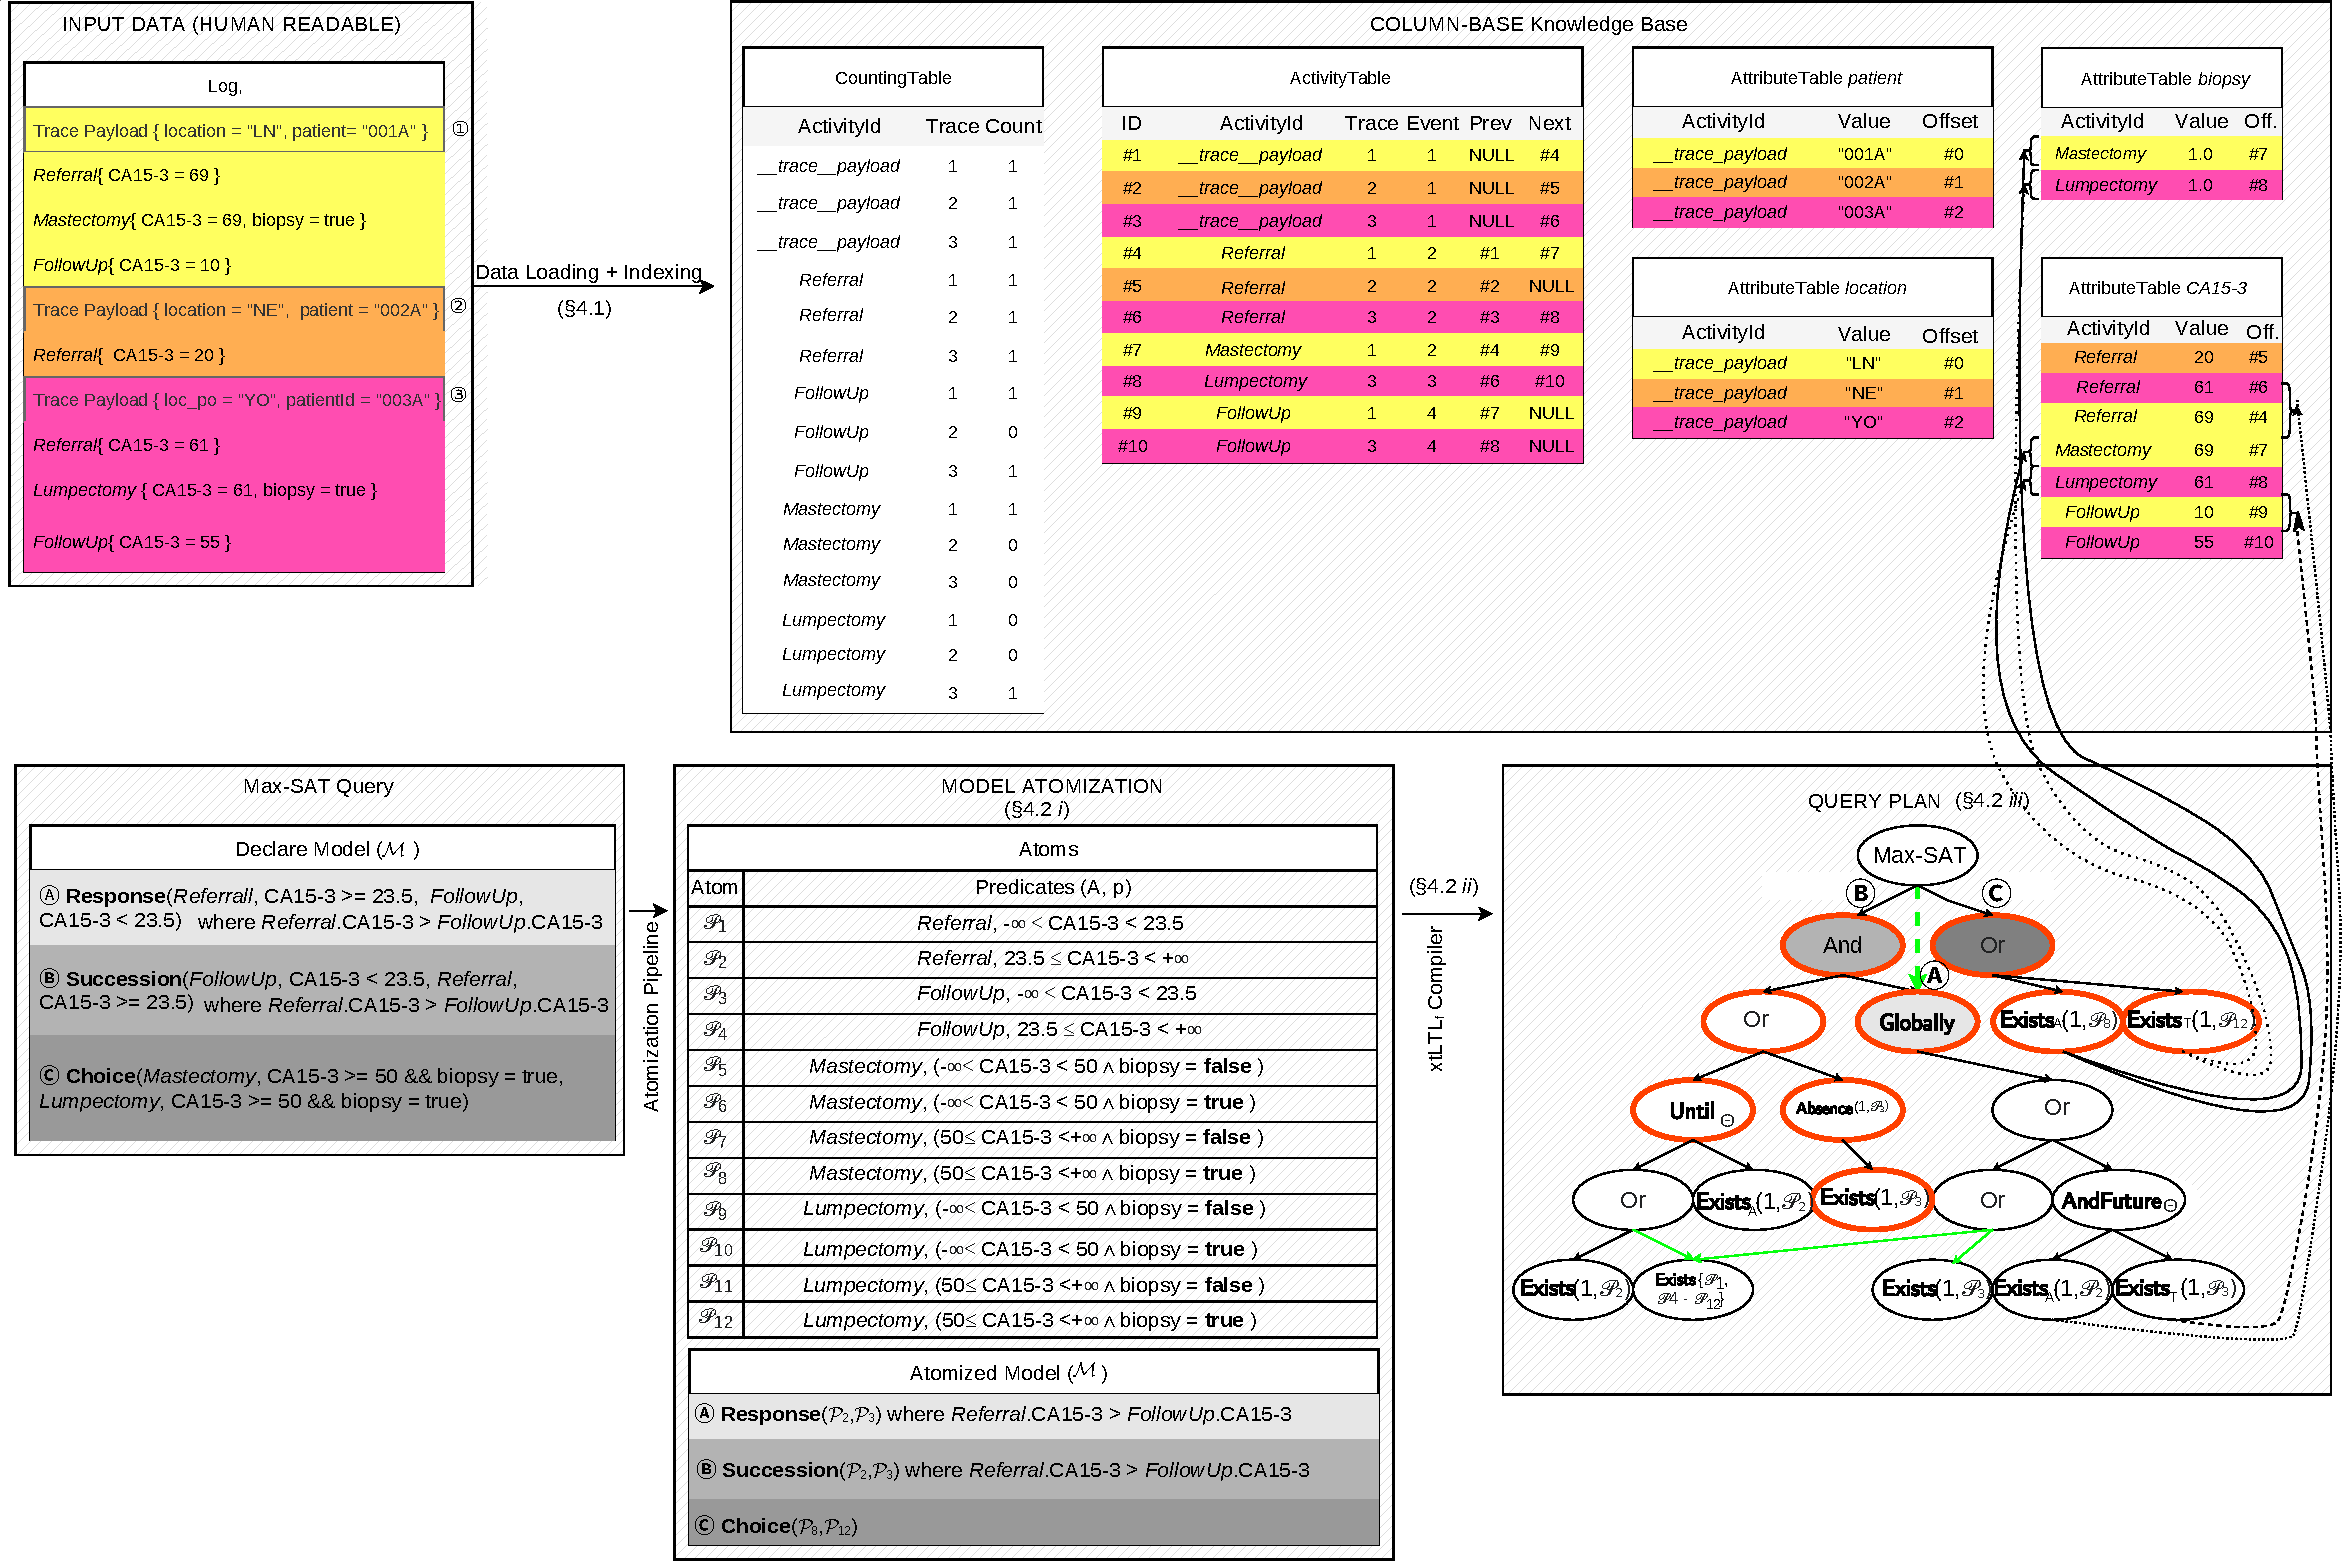
\includegraphics[width=\textwidth]{images/knobab_pipeline.pdf}
	\caption{KnoBAB Architecture for Breast Cancer patients. Each trace \ding{192}-\ding{194} represents one single patient's clinical history, are represented with unique colouring. Please observe that the atomization process does not consider data distribution but rather partitions the data space as described by the data activation and target conditions. In the query plan, green arrows remark access  to shared sub-queries as in \cite{BellatrecheKB21}, and thick red ellipses remark which operators are untimed. } \label{fig:knobab_pipeline}
\end{figure*}
Conformance checking with declarative models
%{Despite the two approaches are equivalent} , {the latter is rather inefficient for conformance checking traces with data payloads} \cite{bpm21}. %Declarative temporal rules are not limited to the mere presence of specific events within the trace, but also determine \RevRepl{how such clauses might occur}{temporal occurrence patterns}. 
{is a well-studied technology at the core} of AI's temporal decision making. \textit{Firstly}, conformance checking is adopted when mining a model from logs either containing only positive (or negative) traces \cite{ROVANI20159236}, or on logs containing both, but where positive traces can be discriminated from the negative ones via behavioural or data conditions, thus allowing to generate both a positive and a negative model  \cite{mining}. 
{The example proposed in this paper (\figurename~\ref{fig:knobab_pipeline}), contains cancer patient records obtained from a hospital (this data is included in our datasets\footnoteref{footnote:datasets}). In healthcare, individuals likely to suffer from an illness should receive treatment, and those that are not suffering should not. Therefore, cases where sufferers not receiving treatment (false negatives) and non-sufferers receiving treatment (false positives) needs to be minimised. \figurename~\ref{fig:knobab_pipeline} proposes a simplified scenario for defining this scenario. We conisder 2 event payload labels: \textsf{CA 15-3} (cancer antigen concentration in a patients blood), and \textsf{biopsy} (biopsies should be taken before any procedure is acted upon). Our model targets only breast cancer patients with successful therapies, that describes a medical protocol and the desired patients' health condition at each step. } %\remove{In a hospital scenario, a positive model might both describe a medical protocol and the desired patients' health condition at each step.} %these might identify the desired health conditions at the end of a medical protocol or simply state the viable solutions.
 %\remove{E.g., For the positive models  in  target only breast cancer patients with successful therapies:}  
 \Circled{\small C} {states} two possible surgical operations for  breast tumours  are  mastectomy or lumpectomy if the biopsy is positive and the CA-13.5 is way above ($\geq 50$) the guard level being 23.5 units per \textit{ml},  and   \Circled{\small A}-\Circled{\small B}  any successful treatment should decrease the CA-13.5 levels, which should be below the guard level; such correlation data condition is expressed via a $\Theta$ condition (also indicated as  \textsf{where}). A twinned negative model (not in \figurename) might better discriminate healthy patients from patients where the therapy was unsuccessful.
%by extracting a declarative model out of a hospital log  containing `successful' traces (e.g., correct procedures, adequate medication), we extract the temporal correlation conditions linking good pre-conditions to expected outcomes  \cite{Amantea2020}. 
\textit{Secondly}, conformance checking can also exploit such models
for predicting which novel clinical situations represented as %on the novel hospital 
traces are likely to adhere to the expected clinical standards. Novel situations can be represented as a log: e.g., in \figurename~\ref{fig:knobab_pipeline}, we have three patients: \ding{192} a cancer patient with a successful mastectomy, \ding{193} a healthy patient, and \ding{194} an unsuccessful lumpectomy, thus suggesting that the patient might still have some cancerous cells. Given the aforementioned model, patient \ding{192} will satisfy the model as the surgical operation was successful, \ding{193} will not satisfy the model because neither mastectomy nor lumpectomy was required {($\mathcal{M}$ is only fulfilled for \textit{successful} procedures)}, and \ding{194} will not satisfy the  target condition, even though the correlation condition was met. Our model of interest should only return %\remove{the first patient}
 {\ding{192}} as an outcome of the conformance checking process.
% \RevRepl{this}{the resulting mined} model \RevRepl{for a current trace to provide the action}{for determining} which \RevAdd{clinical situation} is likely to \RevRepl{be  the next correct decision}{adhere to the expected clinical standards}.



%%\pdfcomment[author=Giacomo]{Please link this description to the infographics, that is going to describe the whole KnoBAB pipeline}
%When a trace does not adhere to the model, we say that the trace is \textit{deviant} \cite{bpm21}. %\RevDel{In the case of traces, the order of the events is important, and temporal information of each event must be stored.}
%E.g., Given a Declare template \textsf{Response}, \DeclareClause{Response}{A}{\textbf{true}}{B}{\textbf{true}} is the instantiated Declare \textit{clause} for \textit{activity labels} \texttt{A} and \texttt{B} stating ``\emph{If event \texttt{A}  happens, event \texttt{B}  must happen either contemporarily or anytime in the future}'' (\figurename~\ref{fig:comparison}); \texttt{A}  (\texttt{B}) is called  \textit{activation} (\textit{target}) condition; a trace would be a deviant \emph{iff.} a trace contained an instance of \texttt{A}  that was not followed by an instance of \texttt{B}. 
%In \figurename~\ref{fig:comparison}, the last trace is the only deviant one. Furthermore, \textbf{true} predicates associated to activation (target) conditions can be enriched to express data conditions (\S\ref{sec:DAD}). As any declarative language, the specification of such templates can be expressed as expressions of logical operators: in this field, Finite Liniear Time Logic (\LTLf) is usually exploited. For instance, clause $\DeclareClause{Precedence}{A}{p}{B}{q}$ becomes $\WeakUntil{\neg(\texttt{B} \wedge q)}{(\texttt{A} \wedge p)}$, %\pdfcomment[author=Giacomo]{Please link this description to the infographics, that is going to describe the whole KnoBAB pipeline} 
%where the binary operator $\WeakUntil{}{}$ denotes that either left-hand-side should always occur until the right- one is found for the first time in the trace, or the left-hand-side should always occur (\figurename~\ref{fig:comparison}). %Activation and target 
%%Conditions might %be 
%%also include % extended with 
%%\textit{correlation} conditions, thus expressing $\Theta$-joins between activated and targeted events. %only between their associated payload. 
%%This is a restriction over traditional relational algebra operators, as we are only interested in analysing such correspondence. %Figure \ref{fig:comparison} exemplifies such intuition.
%%%%{\color{red}[TODO: replace] To further decompose these clauses, algebraic notation can be used to represent the set of operators that are the constituents of a given clause. Declare templates can be represented using \LTLf \cite{Li2020}. This allows for a flexible conformance checking implementation, as each clause can be represented as a unique pairing of \LTLf operators and join operators, for insatnce $\mathbf{RespondedExistence(A,B)}$ becomes $\Future(A) \Rightarrow \Future(B)$\PopUpComment{Giacomo}{Please observe that mathcal should be used only by surrounding the symbol of interest. Otherwise, in some other scenarios, you might have faults. Still, we are going to use a box/diamond notation for this paper. I added some macros for that}. As part of the process mining pipeline, conformance checking is used to identify patterns emerging from a given log. Therefore, process mining can actually be reduced to a conformance checking problem.}\PopUpComment{Giacomo}{Some of the contents in here are good, and should be put elsewhere in the introduction. "In fact, despite these operators might be applied to query plans similarly to relational algebra operators, no work -- to the best of our knowledge -- exploited this possibility". But, this should be linked to another kind of problem, too!}



%\paragraph*{Why do I want to talk about this problem? Why is it relevant?} \textit{Because current literature is lacking of a given aspect} 
%\section{Motivating Example}\label{sec:mot}
%Correlations might be also exploited in 
Real business use case scenarios usually require $\Theta$-correlations. In a goods brokerage scenario \cite{PetermannJMR14},  items are traded between producers (vendors) and retailers (customers): each transaction starts with a vendor sending a sales quotation to a customer. If an offer is accepted and the order is confirmed, then the item is scheduled for delivery. When ready, a logistic operator collects it. %The 
%sales invoice and the sales order is then sent to the retailer. Next, both the producers and the retailers might rank the items on a scale from 0 to 10, where 0 denotes a despicable product while 10 denotes an excellent one. A retailer ranking a product extremely low can file a complaint ticket to the brokerage company which might grant a refund.
In this scenario, deviant traces %are %traces that 
either do not reflect the company's rules or %traces that 
will potentially lead to retailers' complaints: %In particular, a company must send a product only after receiving the offer's acceptance. \dfrac{num}{den}
e.g., % business rule explicitly requiring correlations is the following:   
a late delivery complaint can occur only if the date the product is received is greater than the agreed time to receive it as registered in a previous agreement event. This situation cannot be directly expressed as a temporal pattern, as we also need to test the timestamps associated in the data payload. %Albeit this task requires to represent temporal information within the data perspective \cite{MultiPerspective}, this would require to express \textit{correlation} conditions (\S\ref{sec:DAD}) within the single Declare template of interest. 
%
%\paragraph*{Who might be interested in our solution? How these people might use this work?} \textit{Please provide the pieces of information that are specific to your own research field, and provide some use case examples motivating the practicality of your approach}  
%
{Conformance checking can be applied to several unexplored non-business domains, such as smart contract verification \cite{10.1007/978-3-031-08421-8_9}.} 
% \textit{First}, given that process model information can be exploited to represent 
%  tasks performed by both physical and cybernetic agents \cite{Ioanna}, %this information can be exploited to detect
%   \textbf{cyber-security attacks} can be detected through a model extracted from previous historical data, where specific attacks of interests are selected \cite{BENASHER201551,LagraaS20}. Then, the conformity of any trace to the model might be exploited for determining whether an attack occurred or not. \textit{Second}, \RevRepl{Mining particular patterns within this data }{temporal models extracted from} hospital logs, consisting of diagnoses and treatments with their respective outcomes, could aid \textbf{healthcare} professionals in \RevDel{future} \textbf{decision making} \cite{Amantea2020}. Such models enable explainable AI by associating a precondition to a consequence within a  clinical event of interest \cite{mining,KusumaKMHGJ20}. Conformance checking tools might then assess whether the specific clinical case abides to the declarative rules in the mined model, thus allowing the prediction of a specific clinical event of interest. \textit{Last}, 
   Most recent \textbf{video games}  exploit AI features \cite{LiGT21}: existing state of the art exploits automata \cite{Miyake2017} for modelling \textsc{Non-Player Character}'s behaviours. As Declarative models and automata are completely equivalent approaches, developers might exploit the former to  compactly represent the latter. Furthermore, as debugging AI in video games is a crucial challenge \cite{john2019debugging}, conformance checking solutions might be exploited for debugging unexpected behaviours. As AAA video games already  track and log both players and NPC actions\footnote{\url{https://battlefieldtracker.com/}}, it might be also possible to use game logs for distinguishing winning strategies from losing ones \cite{mining}. As a result, analysis of an ongoing trace at runtime might `suggest'  actions beneficial to the player based on the game state.%, with the current strategy they are pursuing.

%\begin{itemize}
%	%\item A cyber-security attack, where a model can be extracted from previous invasions allowing common patterns to be identified. Some solutions such as \cite{BENASHER201551} use technologies to identify this, but they do not use conformance checking. 
%	\item A hospital log \cite{Amantea2020} [\dots]  \MarkText{In addition to the process discovery, these approaches are `opening the way to perform conformance checking and enhancement', which further justifies our argument that a process mining technique can be reduced to a conformance checking problem.} \PopUpComment{Giacomo}{The problem with this is that it does not explain how this could be done. We shall discuss this in person. Please see the above rephrasing.}
%	%\item Suggesting actions to players in video games. Conformance checking applications for AI in video games has not previously been research; existing state of the art \cite{Miyake2017} use either automata or machine learning. Process mining would allow models to be extracted that represent unique strategies players have attempted in the past. Information regarding their `success' can also be stored. As a result, analysis of an ongoing trace at runtime would then allow the model to `suggest' an action that is beneficial to the player based on the current state of the game, with the current strategy they are pursuing.
%\end{itemize}




\iffalse
%\paragraph*{What do I want to say (to the research community), precisely.} \textit{I want to communicate the general problem that I am aiming to solve} 
Current state of the art conformance checking solutions do not exploit the benefits of storing data in a custom relational database. When running queries, the same data is often accessed multiple times \cite{BurattinMS16,bpm21}. This is especially the case in the process of data-mining with large workloads \cite{SchonigRCJM16}, where the identification of patterns often share similar subqueries. On the other hand, Existing solutions \RevDel{, such as} \cite{BellatrecheKB21}\RevDel{, exploit this by} identify\RevDel{ing} \RevRepl{the}{common} sub\RevAdd{-}expressions within \RevRepl{a query}{several queries running contemporarely}\RevDel{ occurring more than once}, therefore \RevRepl{requiring only one computation}{reduce both the data access and the computation overhead to a minimum.} \RevAdd{This can be easily relate to the conformance checking problem, where multiple declarative clauses from the same model might be assessed contemporarily}. By decomposing these queries into \LTLf, a similar approach can also be followed. We propose that the queries, decomposed into \LTLf operators, can also follow a query plan similar to \cite{BellatrecheKB21}. We extend the approach by adapting the query plan to \RevRepl{use relational algebra with}{express \LTLf operators similarly to relational algebra operations}, where common sub-expressions can still be rationalised. Still, there is some prior work on \RevDel{Another approach proposes a solution that} decompos\RevRepl{es}{ing} clauses into traditional SQL queries \cite{SchonigRCJM16}. This solution \emph{does} exploits the benefits of using a relational database (and therefore query plans) by transforming declare clauses into traditional SQL queries. However, this solution is limited as it \RevRepl{does not}{neither} consider\RevAdd{s} data conditions (only event identifiers), \RevAdd{nor considers multiple clauses pertaining to disparate Declare templates}. This provides less functionality than we propose, where we are data-aware and theta conditions can be taken into account when performing any operators.



%Last, we can observe that some temporal information cannot be expressed by data-agnostic Declare templates. For example, a late delivery complaints occur if the date of a product is greater than the agreed time to deliver it in the previous sales order. This situation cannot be directly expressed as a $\textsf{Precedence}$, as we also need to test the timestamps as both data and event timestamps. Albeit this task requires to represent temporal information within the data perspective \cite{MultiPerspective}, this would require to express \textit{correlation} conditions (see \S\ref{ssec:dad}) within the single Declare template of interest. In the present work, we discard the possibility of expressing such correlation constraints: please observe that this is a quite common consideration within the spectrum of Business Process Management, and therefore we will continue to work under this working assumption \cite{10.1007/978-3-642-40176-3_8}. Nevertheless, we are planning to extend the proposed approach so to perform conformance checking containing correlation constraints. 
%Conformance checking is an integral part of artificial intelligence that bridges data mining and business process management. 


%Conformance checking can be extremely computationally intensive, both in time and storage, so optimised solutions are necessary to ensure a well performant implementation. To our knowledge, no solution existing whereby a relational base exploits optimised query plans, adapting solutions such as \cite{BellatrecheKB21}, in a business process environment using LTLf.
\medskip


\paragraph*{Now, communicate our idea also to the people working in our same area!} \textit{In particular, this means that we can go down in technicalities on what we want to solve, which are the primarily goals of our research, and which are the intermediate requirements/results leading to the results that we expect.} 
Assessing the ability of each trace to satisfy a given temporal logical constraint is computationally costly: intuitively, checking whether a \textsf{Response} condition is met in a trace will require the possibility of tagging those with event distinctive labels, and to evaluate if the condition holds by joining each possible event A in the temporal series with the B events happening in the future, if any, and counting if all of the A events within the series satisfy such criteria. As we might see, this might become quite costly in big data scenarios, where both traces' lengths and their number is considerable high. If we want to also list all of the traces satisfying this condition, this computational burden is worsened by the costly \texttt{Group By} operation on traditional data bases, thus including document-oriented ones \cite{THoSP}.

As process mining can be reduced to a conformance checking problem, a given log can be queried against a declarative model at runtime, and the same conformance checking calculations can be applied to generate its conformance \emph{at the current time}. Therefore, KnoBAB provides an optimized representation of the trace logs over which the declarative models $\mathcal{M}$ are going to be both queried and mined with \LTLf.

We propose a knowledge base, KnoBAB, which provides efficient conformance checking by adapting query plan optimisations \cite{BellatrecheKB21} to \LTLf. In addition, we provide data-aware capabilities, which discussed database solutions do not. KnoBAB provides the conformance of a \emph{trace} to a set of clauses, not the conformance of a clause against a log. This is more valuable in scenarios where trace information could point to where, and why, it was a deviant. Such knowledge could then be used for many features, such as generating the repair for this trace.
\medskip


The greatest amount of performance gain is due to the custom query plan, structured in such a way that multiple queries are stored within a graph, and then batch jobs are run using \textbf{parallelisation}. When process mining, large numbers of queries are performed, therefore there will be many instances of duplicate data accessing, resulting in poor optimisation. In this approach, there is the guarantee that unique data elements are obtained and processed only once, while current state of the art process-mining approaches access data per query. 
\fi


Given that conformance checking is at the heart of both trace validation and model mining, it is of crucial relevance to optimize such a task.
Solutions enabling conformance checking via model mining through SQL queries \cite{Schonig15,SchonigRCJM16}  neither explicitly evaluate the satisfiability for every single trace, nor return the traces that satisfy them, but only associate support and confidence values to each of said clauses for model mining purposes. However, as shown in this paper,  these queries can be extended to both 
evaluate satisfiability per trace and return the set of traces satisfying every single clause, thus adhering to the definition from conformance checking literature (\S\ref{sec:DAD}). In doing so,  we are forced to introduce  aggregation and nesting operations, which are not generally efficient. This fact is supported by experimental evidence (\S\ref{ssec:sqlmin}), where we also extend the relational representation of traces from \cite{Schonig15,SchonigRCJM16} (\S\ref{ssec:dl}). Our specific contribution is then the provision of specific operators (\xLTLf) rewriting existing \LTLf operators for the relational  model thus efficiently running conformance checking queries in Declare (\S\ref{sec:xltlf}). This is also possible through a query plan solution similar to  \cite{BellatrecheKB21} (\S\ref{ssec:xltlf}), which  proves to be more efficient than any solution relying solely on the SQL language. {The Query Plan (\figurename~\ref{fig:knobab_pipeline}), utilises our proposed \xLTLf operators (\S\ref{sec:xltlf}), as an extension of the traditional \LTLf operators (\S\ref{sec:DAD}) that logically define a Declare clause (\tablename~\ref{tab:dt}). While \LTLf operators provide a formal logical temporal definition, \xLTLf operators are designed to exploit the benefits that a relational model provides. This includes optimized access to the tables defined in \figurename~\ref{fig:knobab_pipeline}. For example, the proposed operator \textsf{Init}, which constrains a log to begin with a specified event, can directly access the \textsf{CountingTable}, and exploit offsets to determine the first event per trace. Traditional \LTLf (used for a relational model) would require an entire log scan. }

Even state-of-the-art implementations explicitly engineered to solve the conformance checking problem without relying on a 
relational representation of traces, are not particularly efficient \cite{BurattinMS16}. This solution, not being able to assemble the previously described \LTLf operators within a query plan, can neither minimize the access operations to the trace data nor  minimize the re-computation of sub-expressions that appear frequently in the model as recently proposed by \cite{BellatrecheKB21}. This claim is also supported by analysing the query plan for more recent approaches where no evidence of query optimization over the query plan is given \cite{Polyvyanyy2022,MurillasRA22}. Further experimental shreds of evidence support such theoretical claims (\S\ref{ssec:declan}): in the first instance, these show that our solution is already more efficient than the state of the art in the literature by two{-three} orders of magnitude (hundredths{\textbackslash tenths} of a millisecond vs. tens of seconds). Furthermore, by using different Declare models composed of several clauses accessing the same activation and target conditions, except the data correlations, our solution exhibits an increase in running time only when new data is accessed and, otherwise, it preserves a constant running time with fewer temporal fluctuations.

%{\subsection{Contributions}}
\paragraph*{Contributions} Our proposed solution is then implemented in KnoBAB\footnote{\url{https://github.com/datagram-db/knobab}}: we are synthesising logs derived from a system (be it digital or real) to a column-store knowledge base ad-hoc implemented for conformance checking (\S\ref{ssec:dl}). In this instance, we then generate a conformance checking query plan generated from a declarative model (\S\ref{sec:qc}), be it positive or negative, so to compute desired properties associated with non-deviant traces (\S\ref{ssec:xltlf}). As per previous remarks, declarative models represent temporal and data constraints that one would expect to hold as true in the non-deviant traces from the twinned system. As such, one can consider those traces returned by the query associated with the declarative model as correct, and the remainder as deviant. As a temporal representation of the declarative model provides a point-of-relativity in the context of correctness (i.e., time itself may dictate if traces maintain correctness throughout the unfolding of the associated events), the considerations of such temporal issues significantly increase the time spent for checking the meeting of the requirements.  Our contributions include: 
%\remove{first, we show how to extend the relational solution for representing logs from \mbox{\cite{Schonig15,SchonigRCJM16}} with a \textsf{CountingTable} and a column-based relational model for representing data payloads (\mbox{\S\ref{ssec:dl}}, upper part of \mbox{\figurename~\ref{fig:knobab_pipeline}}). Second, we design a query compiler (\mbox{\S\ref{sec:qc}}) transforming each Declare model composed of multiple single clauses into a DAG query plan (lower part of \mbox{\figurename~\ref{fig:knobab_pipeline}}). Next, we designed an execution engine running the \mbox{\xLTLf} operators either sequentially or in parallel (\mbox{\S\ref{ssec:xltlf}}).}
{\begin{enumerate*}[label=(\textit{\roman*})]
	\item an extension of the log representation from \cite{Schonig15,SchonigRCJM16} with a \textsf{CountingTable} and a column-based relational model for representing data payloads (\S\ref{ssec:dl}, upper part of \figurename~\ref{fig:knobab_pipeline}),
	\item a query compiler (\S\ref{sec:qc}) transforming each Declare model into a DAG query plan (lower part of \figurename~\ref{fig:knobab_pipeline}),
	\item a relational formulation of traditional \LTLf as \xLTLf, and
	\item an execution engine running the DAG either sequentially or in parallel (\S\ref{ssec:xltlf})
\end{enumerate*}}
